%!TEX root = ../document.tex

\section{Método de Rocha et al.}
\label{sec:section2}
Este método é baseado em dois pontos-chave: (i) medida do desvio ST através de análise tempo-frequencial do ECG e (ii) expansão do complexo QRS e da onda T em funções de Hermite. A figura \ref{fig:rocha_01} mostra o diagrama em blocos da estratégia adotada. A implementação dos procedimentos de cada etapa é detalhada a seguir.

\begin{figure}[h]
    \centering
    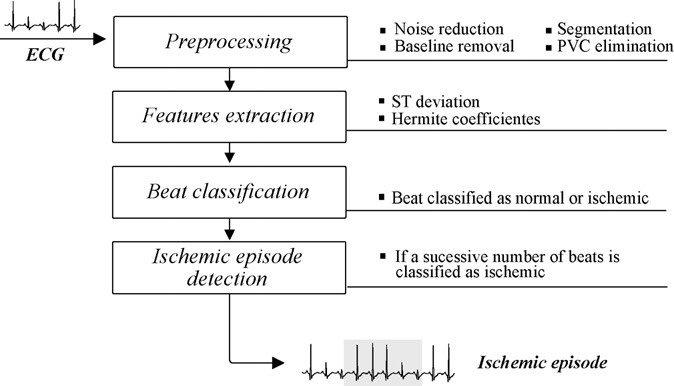
\includegraphics[width=0.8\textwidth]{figures/rocha_01.png}
    \caption{Diagrama de blocos da estratégia utilizada no método de Rocha et al. Extraído de \cite{Rocha10}}
    \label{fig:rocha_01}
\end{figure}

\subsection{Pré-processamento}
Nesta etapa, um sinal de entrada discreto contendo as amplitudes normalizadas\footnote{aqui, normalizado significa $(Amplitude - Deslocamento) / Ganho$} de um ECG é processado para redução de ruído, segmentação em ondas características, eliminação de extra-sístoles ventriculares e, por último, remoção da linha de base.

Para redução de ruído, o sinal é filtrado usando um filtro passa-baixas de Butterworth. Os parâmetros do filtro são: ordem 4 e frequência de corte 40Hz. O sinal filtrado é então submetido a um procedimento de segmentação, em que as ondas características de cada batida são identificadas. Seguindo a especificação, utilizou-se um algoritmo descrito em \cite{Sun05}. Na saída obtêm-se as localizações de início, pico e fim de cada onda característica no eixo temporal.

Após a segmentação, cada batida é classificada como normal ou extra-sístole ventricular (também chamada PVC, do inglês \emph{premature ventricular contractions}). Utiliza-se para este processo o algoritmo proposto em \cite{Couceiro08}. As PVCs são então removidas da lista de batidas do ECG, e somente aquelas classificadas como normais serão analisadas nas etapas posteriores.

O último procedimento nesta etapa consiste em extrair do sinal de ECG a linha de base, e subtraí-la do próprio sinal afim de torná-lo mais ``limpo''. Isso é necessário para as próximas etapas, pois alguns procedimentos exigem que as batidas estejam bem alinhadas com o nível de amplitude zero.

\subsection{Extração de características}
Nesta etapa, dois grupos de características são extraídos do ECG, quais sejam, medida do desvio de segmento ST e expansão de Hermite do complexo QRS e das ondas T. Variações no desvio do segmento ST, medido a partir da linha de base, são usadas para discriminar batidas isquêmicas de batidas normais. De maneira similar, variações na morfologia do complexo QRS e da onda T indicam presença ou não de isquemia.

Duas medidas de desvio do segmento ST são obtidas através de dois métodos distintos, e compõem o primeiro grupo de características usadas na classificação. Um método é baseado na localização dos picos de onda R, de acordo com o algoritmo proposto em \cite{Pang05}. O outro é derivado de uma análise em tempo-frequência do ECG usando a transformada de Wigner-Ville, conforme descrito abaixo.

\subsubsection{Transformada de Wigner-Ville}
Explicação do método de medida do desvio de segmento ST baseado na transformada de Wigner-Ville\ldots

\begin{equation} \label{equ:wigner_ville}
    W_x(t,f) = \int_{-\infty}^{\infty} x\left( t+\frac{\tau}{2} \right) x^*\left( t-\frac{\tau}{2} \right) e^{-j2\pi f \tau} d\tau
\end{equation}

\begin{equation} \label{equ:pseudo_wigner_ville}
    W_x(nT,f) = 2T\sum_{-L}^{L}x(n+p)x^*(n-p)w(p)w^*(-p)e^{-j4\pi f\tau}
\end{equation}

\subsubsection{Expansão de Hermite}
Para o segundo grupo de características, os autores propuseram uma técnica baseada em funções de Hermite. Uma função de Hermite de ordem $n$ pode ser expressa como o produto de uma Gaussiana com um polinômio de Hermite, conforme a equação abaixo.
\begin{equation} \label{equ:hermite_function}
    H^n(t,l) = \frac{e^{-t^2/2l^2}}{\sqrt{n!2^n\sqrt{\pi}l}}p^n\left(\frac{t}{l}\right)
\end{equation}
onde $p^n$ é o polinômio de Hermite de ordem $n$ e $l$ é um fator de escala.

Usando esta definição, e sabendo que as funções de Hermite formam uma base para o espaço de funções integráveis ao quadrado ($L^2$), é possível aproximar um sinal discreto por uma expansão em funções de Hermite. A expansão consiste em obter uma lista de coeficientes que satisfazem a equação abaixo.
\begin{equation} \label{equ:hermite_expansion}
   \hat{y}(k) = \sum_{j=0}^{m-1} c_jH^j(k,l)
\end{equation}
onde $c_j$ é o coeficiente da $j$-ésima função de Hermite e $m$ é o número de funções utilizadas na aproximação. Os coeficientes são solução da equação abaixo.
\begin{equation} \label{equ:solve}
    C = (H^TH)^{-1}H^TY
\end{equation}
onde H é uma matriz formada pelas funções de Hermite
\begin{equation}
    H = [H_0\ H_1\ \cdots\ H_{m-1}]
\end{equation},
C é um vetor coluna contendo os $m$ coeficientes de Hermite
\begin{equation}
    C = [c_0\ c_1\ \cdots\ c_{m-1}]^T
\end{equation}
e Y é um vetor coluna de tamanho $n$ contendo as amplitudes do sinal de entrada.

No algoritmo proposto, são consideradas as primeiras 6 funções de Hermite, e o sinal de entrada é separado em dois componentes: um contendo as amostras do complexo QRS e outro contendo as do segmento ST juntamente com as da onda T. Dessa forma, para cada batida, dois conjuntos de amostras são submetidos ao procedimento de expansão de Hermite, e a saída nos fornece uma lista de 6 coeficientes para o primeiro conjunto (QRS) e uma lista de 6 coeficientes para o segundo (ST-T).

